% 2011 年湖南卷理科第 19 题：圆锥 PO，C 为半圆 AB 中点，D 为 AC 中点。
% 来源 PDF：普通高考/2011/2011湖南理.pdf，SHA-256 09b67f1db8e6a280165cf8431211a968163c0d0f262a50068dd607607a9ec578。
% 原页：第 2 页第 1 栏下部，书页码 672。示意。
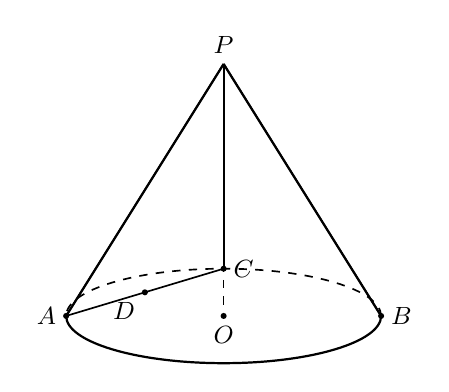
\begin{tikzpicture}[>=stealth, semithick, font=\small, scale=1.0]
  \draw[thick] (0,3.2)--(-2,0);
  \draw[thick] (0,3.2)--(2,0);
  \draw[thick] (-2,0) arc (180:360:2 and 0.6);
  \draw[dashed] (2,0) arc (0:180:2 and 0.6);
  \draw[dashed] (0,3.2)--(0,0);
  \coordinate (A) at (-2,0);
  \coordinate (B) at (2,0);
  \coordinate (C) at (0,0.6);
  \coordinate (D) at (-1,0.3);
  \draw[thick] (0,3.2)--(C);
  \draw (A)--(C);
  \draw (0,3.2)--(A);
  \draw (0,3.2)--(B);
  \fill (A) circle (1.1pt) node[left] {$A$};
  \fill (B) circle (1.1pt) node[right] {$B$};
  \fill (C) circle (1.1pt) node[right] {$C$};
  \fill (D) circle (1.1pt) node[below left] {$D$};
  \fill (0,0) circle (1.1pt) node[below] {$O$};
  \node[above] at (0,3.2) {$P$};
\end{tikzpicture}
